\subsection{Logic Synthesis}
The synthesis of the circuit was done with the Synopsys software. The first objective is to determine the maximum frequency that will allow the correct operation of the circuit and its area. The standard port libraries provided have been used to automatically synthesize even the complex logical blocks such as adders and multipliers.
In a preliminary phase a clock with period $T_{clk} = \SI{10}{\nano\second} \pm \SI{0.07}{\nano\second}$ has been set. The result of the synthesis shows a slack of $+\SI{5.14}{\nano\second}$; the fact that the slack is positive implies that the clock constraints set have been met with the synthesis obtained.
To evaluate the maximum operating frequency of the circuit, a clock period of 0 has been set, so theoretically the negative slack obtained should correspond to the minimum necessary clock period. However, this is only partially true, since setting the clock period to the new value will still result in a negative slack. This behavior is due to the fact that the synthesizer changes the structure of the internal slack according to the constraint provided on the clock as you can see from the data on the area. It was necessary to iterate this procedure several times to obtain a slack equal to 0 and therefore the maximum operating frequency of the circuit. In \autoref{tab:timing_rep} a summary of the results obtained is shown.

\begin{table}[h]
\begin{center}
\begin{tabular}{|l|l|l|}
\hline
$T_{CLK}$ (ns) & slack (ns) & area $(\SI{}{\micro\meter})^2$ \\
\hline
10 & 5.14 & 1991 \\
0 & -3.13 & 2491 \\
4.10 & 0 & 2187 \\
16.4 & 11.54 & 1991 \\
\hline
\end{tabular}
\end{center}
\caption{Results of timing report}
\label{tab:timing_rep}
\end{table}

The second goal is to find area and power consumption by setting $T_{CLK} = 4 T_{min}$. For the area you can refer to \autoref{tab:timing_rep}. For the power computation, a record of the switching activity has been generated through a Modelsim simulation and saved on a vcd file, subsequently converted in saif file. The presence of these data serves during the calculation of the correct power consumption in the Synopsys environment. The results are shown in \autoref{fig:pow_rep_x4}.

\begin{figure}[htb!]
	\center
	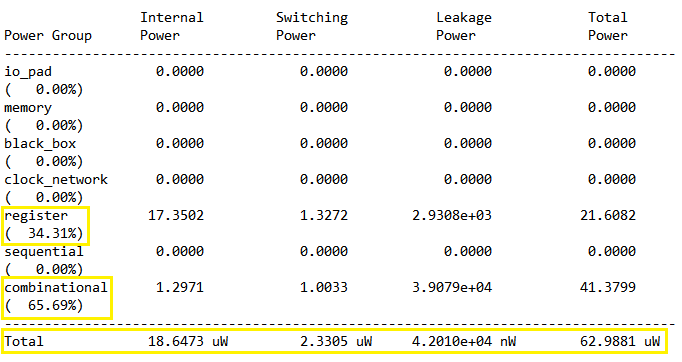
\includegraphics[width=0.8\textwidth]{rep_power_x4_mod.png}
	\caption{Power Report}
	\label{fig:pow_rep_x4}
\end{figure}

It can be seen that the power is divided between the registers and the combinatorial part with a preponderance of this second contribution, $65\%$, due to the presence of 3 multipliers and 2 adders in the designed architecture.

\subsection{Place \& Route}
The last operation is the place and route of the circuit using the Innovus software. The netlist generated by Synopsys with $T_{CLK} = 4 T_{min}$ and the standard libraries have been used as a starting point. After the various required steps the final circuit shown in \autoref{fig:layout} has been obtained.

\begin{figure}[htb]
	\center
	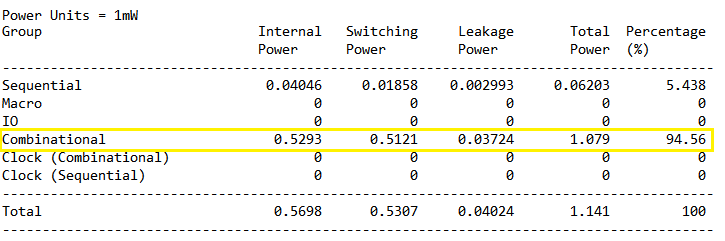
\includegraphics[width=0.7\textwidth]{rep_power_x4_cadence_mod.png}
	\caption{Post place \& route power report}
	\label{fig:cadence_pow_rep_x4}
\end{figure}

\begin{figure}[htb!]
	\center
	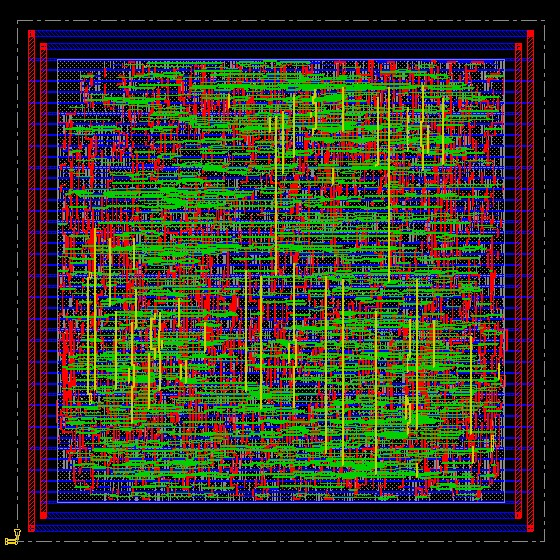
\includegraphics[width=0.5\textwidth]{IIR_filter_period_min_x4_place.jpg}
	\caption{Resulting layout}
	\label{fig:layout}
\end{figure}

The product layout has an area of $\SI{1959}{\micro\meter}^2$, which is in agreement with the estimated Synopsys' estimate shown in \autoref{tab:timing_rep}, with a total of 986 cells and 2455 gates. Then the timing analysis was launched to verify that the timing constraints were correct, then the connectivity and geometry was verified. Finally, using the switching activity calculated with Modelsim, the power consumption has been re-estimated. The results obtained are shown in \autoref{fig:cadence_pow_rep_x4}.


The power values obtained are in agreement with those obtained by Synopsys in \autoref{fig:pow_rep_x4}. Moreover, since the calculation at this level is much more accurate as it takes into account the physical layout of the circuit, it can be seen that in fact the consumption of the combinatorial part is prevalent.